

\begin{frame}{NP-type effect (LMM)}

\begin{tikzpicture}
    \draw (0, 0) node[inner sep=0,anchor=west] {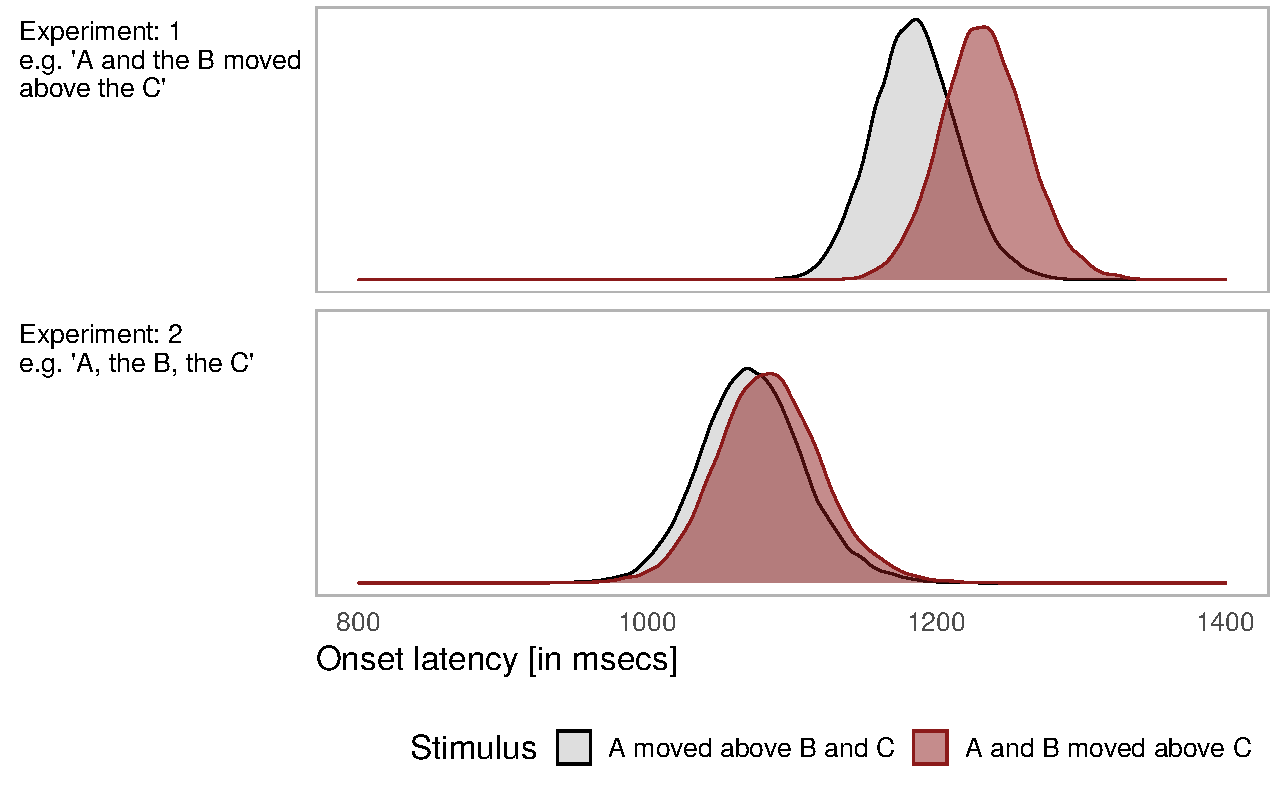
\includegraphics[scale=.5]{NPexp.pdf}};
    \draw (2.75, 2.9) node[font=\tiny,anchor=west] {LMM-1 -- LMM-0: $\updel\widehat{elpd}=$-6 (3)};
    \draw (2.75, 2.5) node[font=\tiny,anchor=west] {LMM-1: $\widehat{elpd}=$-22,125 (78)};
    \draw (10.75, .35) node[font=\tiny,anchor=east] {LMM-1 -- LMM-0: $\updel\widehat{elpd}=$0 (1)};
    \draw (10.75, -.05) node[font=\tiny,anchor=east] {LMM-1: $\widehat{elpd}=$-14,318 (69)};
\end{tikzpicture}

\end{frame}

\begin{frame}{Probability of long latencies (MoG)} 

\begin{tikzpicture}
    \draw (0, 0) node[inner sep=0,anchor=west] {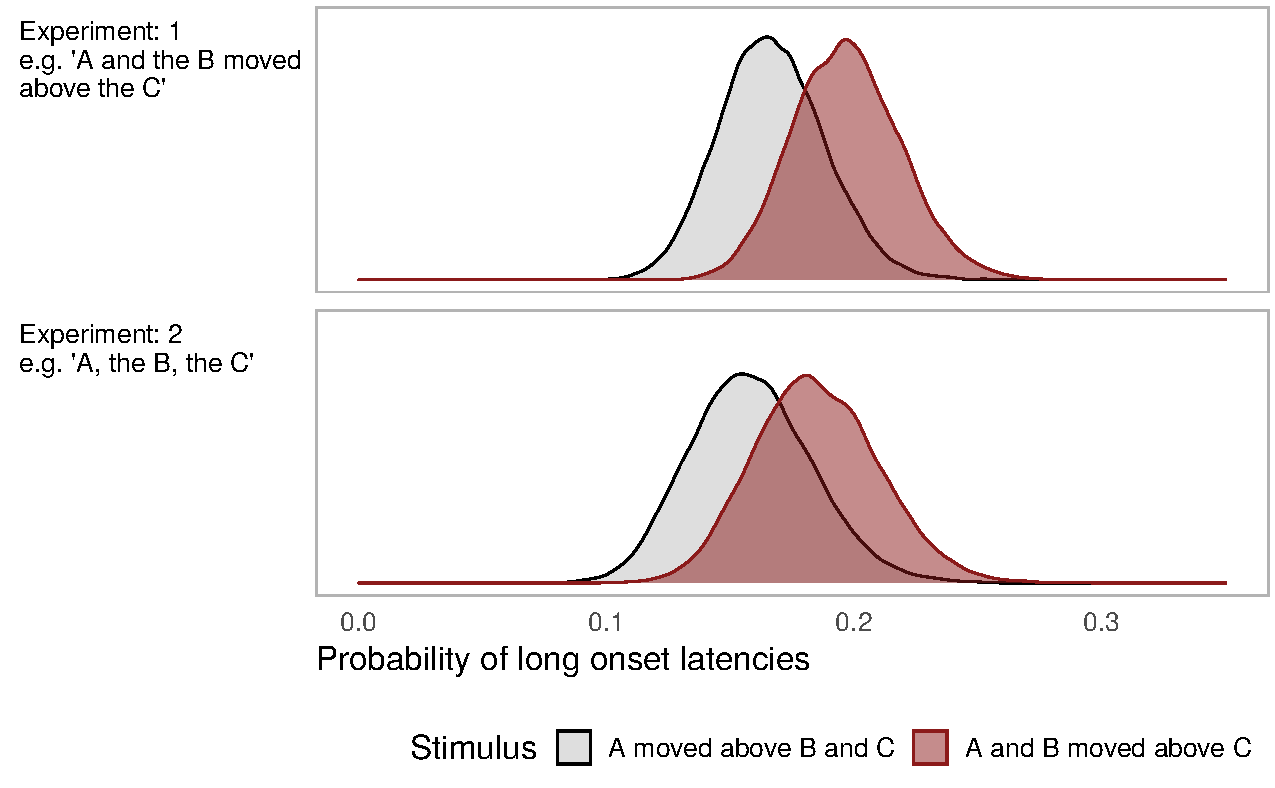
\includegraphics[scale=.5]{NPexpmog.pdf}};
    \draw (10.75, 2.95) node[font=\tiny,anchor=east] {MoG-1 -- LMM-1: $\updel\widehat{elpd}=$-401 (36)};
    \draw (10.75, 2.55) node[font=\tiny,anchor=east] {MoG-1: $\widehat{elpd}=$-21,725 (65)};
    \draw (10.75, .45) node[font=\tiny,anchor=east] {MoG-1 -- LMM-1: $\updel\widehat{elpd}$=-305 (35)};
    \draw (10.75, .05) node[font=\tiny,anchor=east] {MoG-1: $\widehat{elpd}$=-14,013 (54)};
\end{tikzpicture}

\end{frame}
